\begin{figure}[htbp]
\centering
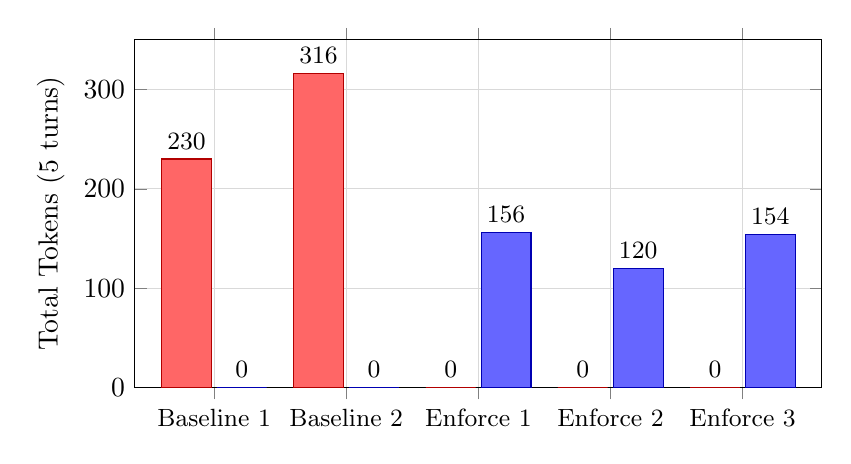
\begin{tikzpicture}
\begin{axis}[
    width=0.85\textwidth,
    height=6cm,
    ybar,
    bar width=18pt,
    ylabel={Total Tokens (5 turns)},
    symbolic x coords={B1, B2, E1, E2, E3},
    xtick=data,
    xticklabels={Baseline 1, Baseline 2, Enforce 1, Enforce 2, Enforce 3},
    x tick label style={rotate=0, anchor=north, font=\small},
    ymin=0, ymax=350,
    nodes near coords,
    nodes near coords align={vertical},
    every node near coord/.append style={font=\small},
    grid=major,
    grid style={gray!30},
    enlarge x limits=0.15,
]

\addplot[fill=red!60!white, draw=red!70!black]
    coordinates {(B1,230) (B2,316) (E1,0) (E2,0) (E3,0)};

\addplot[fill=blue!60!white, draw=blue!70!black]
    coordinates {(B1,0) (B2,0) (E1,156) (E2,120) (E3,154)};

\end{axis}
\end{tikzpicture}
\caption{Total token expenditure across 5 turns. Baseline systems consume 230--316 tokens (growth). Enforcement systems consume 120--156 tokens (compression), a 32--48\% reduction. Enforcement 2 achieves the lowest total at 120 tokens---a 48\% reduction relative to Baseline 1 and 62\% relative to Baseline 2.}
\label{fig:total-comparison}
\end{figure}
